\chapter{Related work}
This chapter is about presenting CellProfiler Analyst (CPA), a first generation tool for interactive 
data exploration and classification of large biological image sets. 
It was first introduced in 2016 at the Broad Institute of MIT and Harvard. 
The following section gives an overview of CPA's main functionality and an exploration of its key features, 
the classifier and image gallery. 

This project is highly influenced by CPA and basically aims to improve it and make it accessible
to anybody without having to install any software. CPA is free and open source, 
available at \href{http://www.cellprofiler.org}{http://www.cellprofiler.org} and from GitHub under a 
BSD-3 license. It is available as a packaged application for
Mac OS X and Microsoft Windows and can be compiled for Linux.

\subsection{CellProfiler Analyst}
CPA is a GUI based tool. It provides features for data exploration and classification via 
its user interface. There are only a few comparable tools for this purpose, the most prominent being  
Ilastik, CellCognition and WND-CHARM.

All these tools lack a suitable companion visualization tool capable of handling large datasets. 
Furthermore they do not provide selectable classifier algorithms. Another big benefit CPA has compared 
to all other existing tools that it incorporates an interactive object classification and image viewing feature.

\begin{figure}[H]
	\centering
	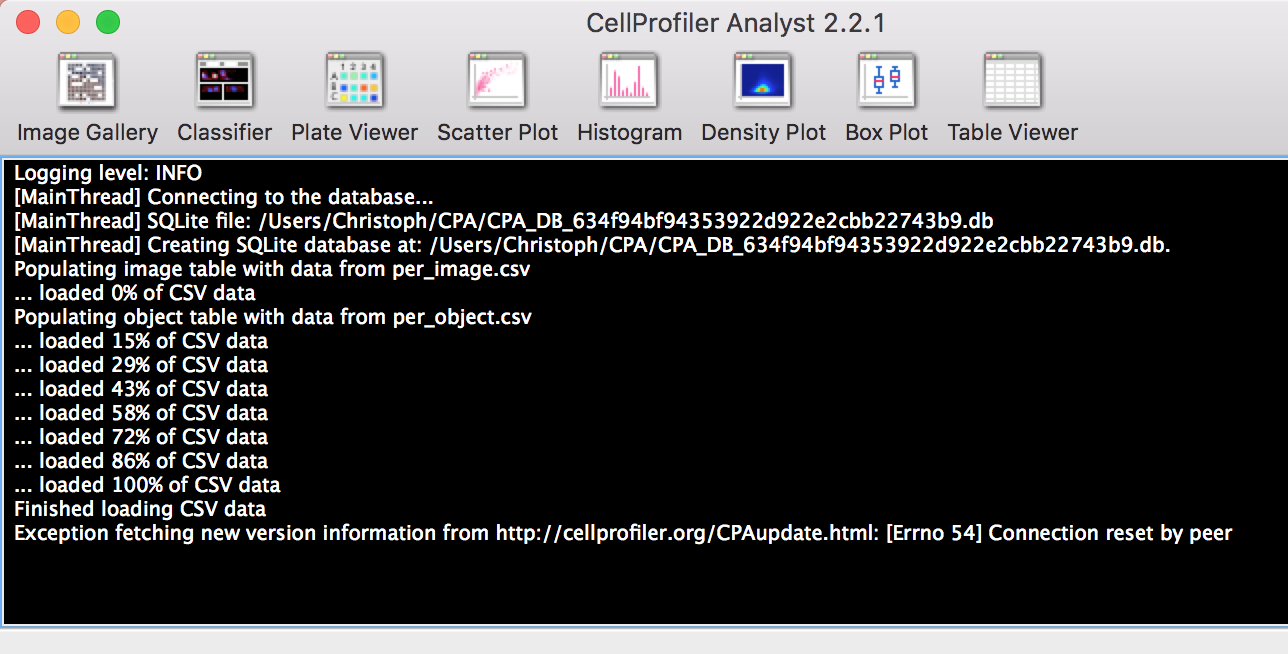
\includegraphics[width=1.0\linewidth]{bilder/related_work/cpa_main_view.png}
	\caption{CPA main view, different views are selectable  (from \cite{Jones2008})}
	\label{fig:CPA}
\end{figure}

\subsection{Classifier}
The Cell Profiler Analyst Classifier makes it possible to create categories and to classify cells.
 After fetching images from a predefined dataset it is possible to classify images 
 by simply drag and dropping them on a category. Multi-select features are also implemented
  and enable to drag and drop multiple images at the same time. 
  
  Further it is possible to add an unlimited amount of categories by clicking the "add category" button. 
  After annotation is done the algorithms can be trained. Once training is done more images can be 
  fetched and then be automatically annotated by clicking the "evaluate" button. 
  
  If results do not suffice further images can be annotated to train the algorithm. 
  Different algorithms can be used to classify the uncategorized images, such as 
  RandomForest Classifier and AdaBoost Classifier.

\begin{figure}[H]
	\centering
	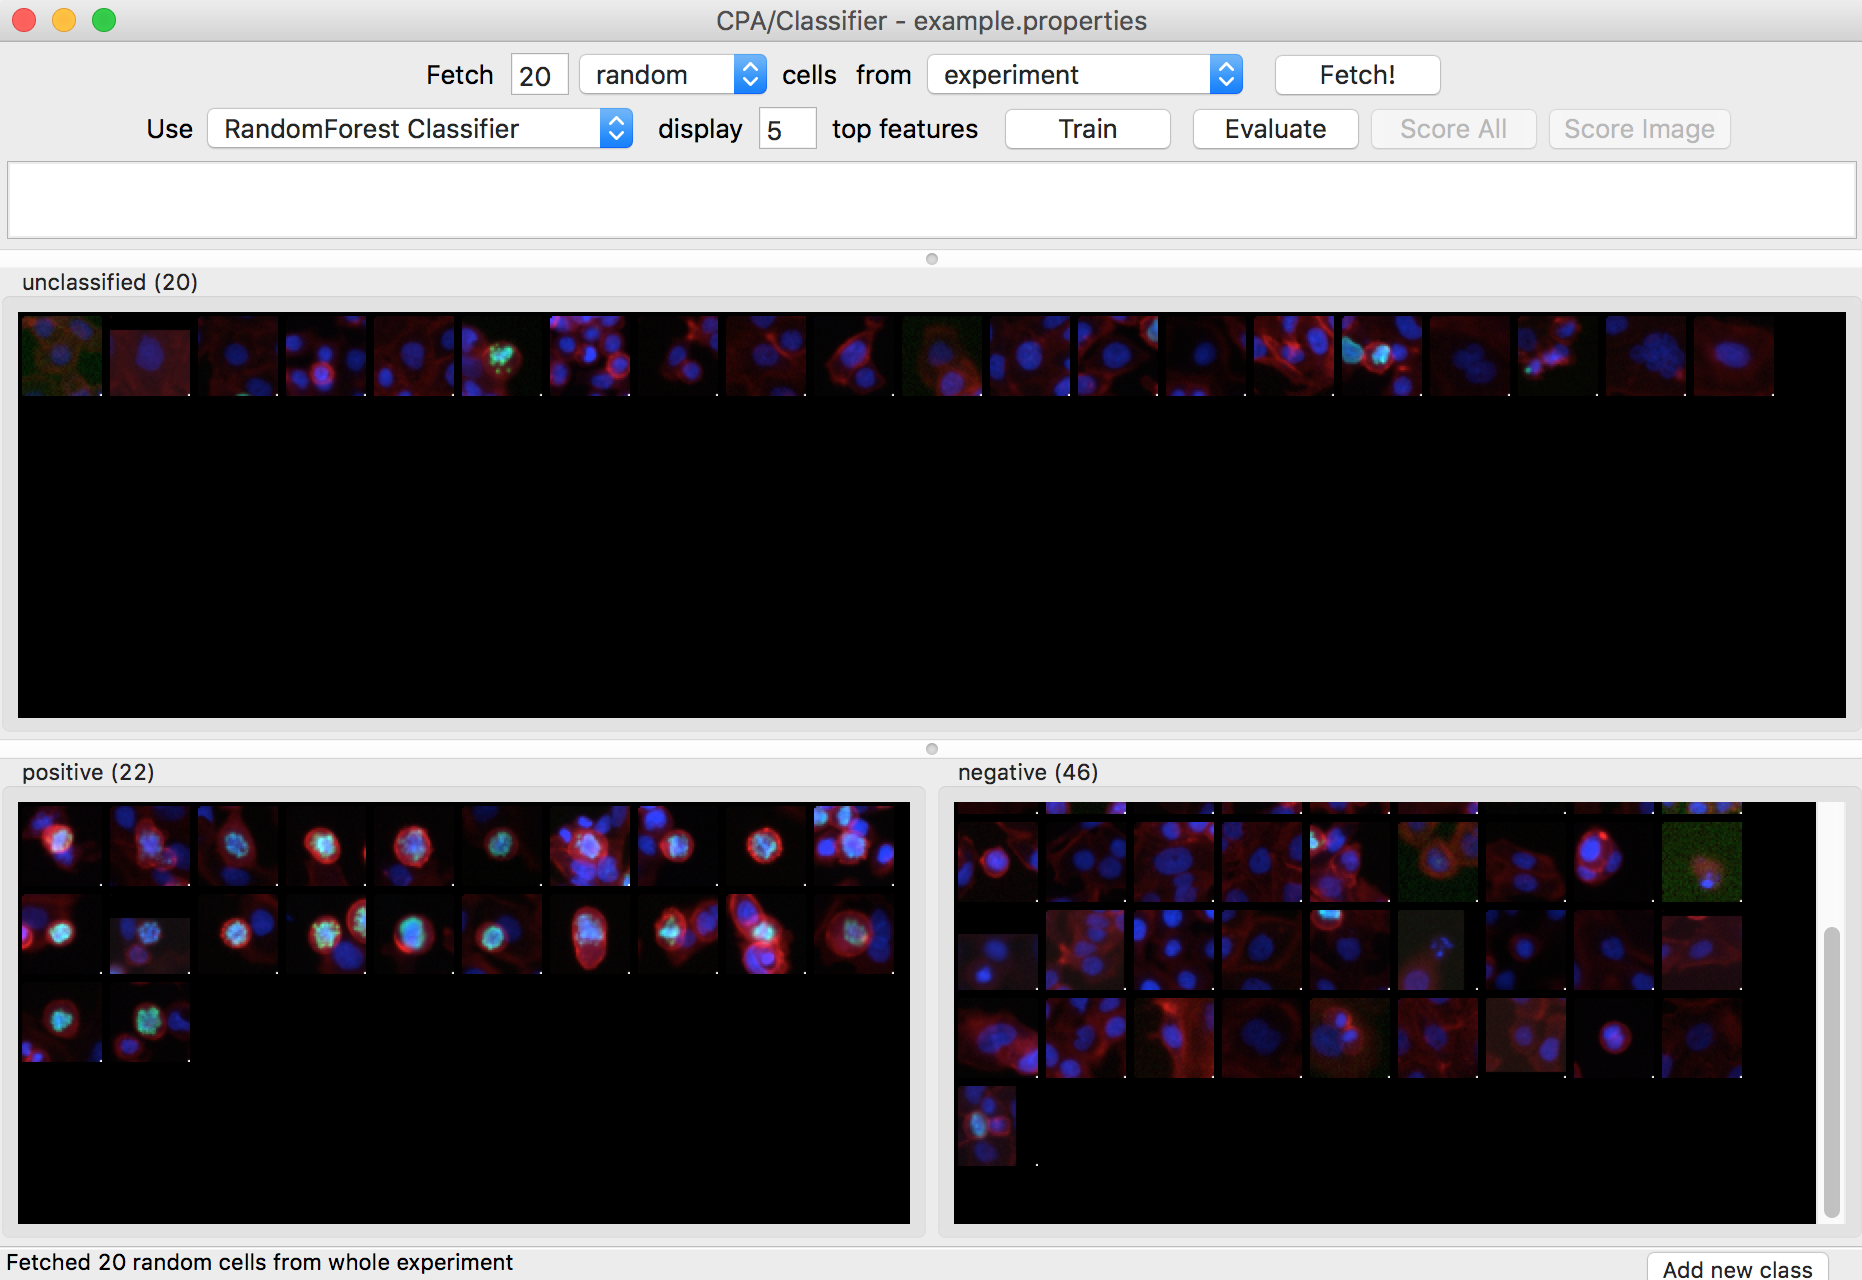
\includegraphics[width=1.0\linewidth]{bilder/related_work/classifier.png}
	\caption{CPA main view. Different views Are Selectable (from \cite{Jones2008})}
	\label{fig:Classifier}
\end{figure}


\subsection{Visualization}


In order to explore a dataset and to predict and validate a result, a good visualization is needed. 
CPA offers different ways of displaying data and results. 

One simple visualization possibility is the Image Gallery where images from the dataset can be selected and 
displayed in their original size. Filters can be applied to only select images with experiment specific meta data. 
There are many more ways to display and explore data in CPA.

\begin{figure}[H]
	\centering
	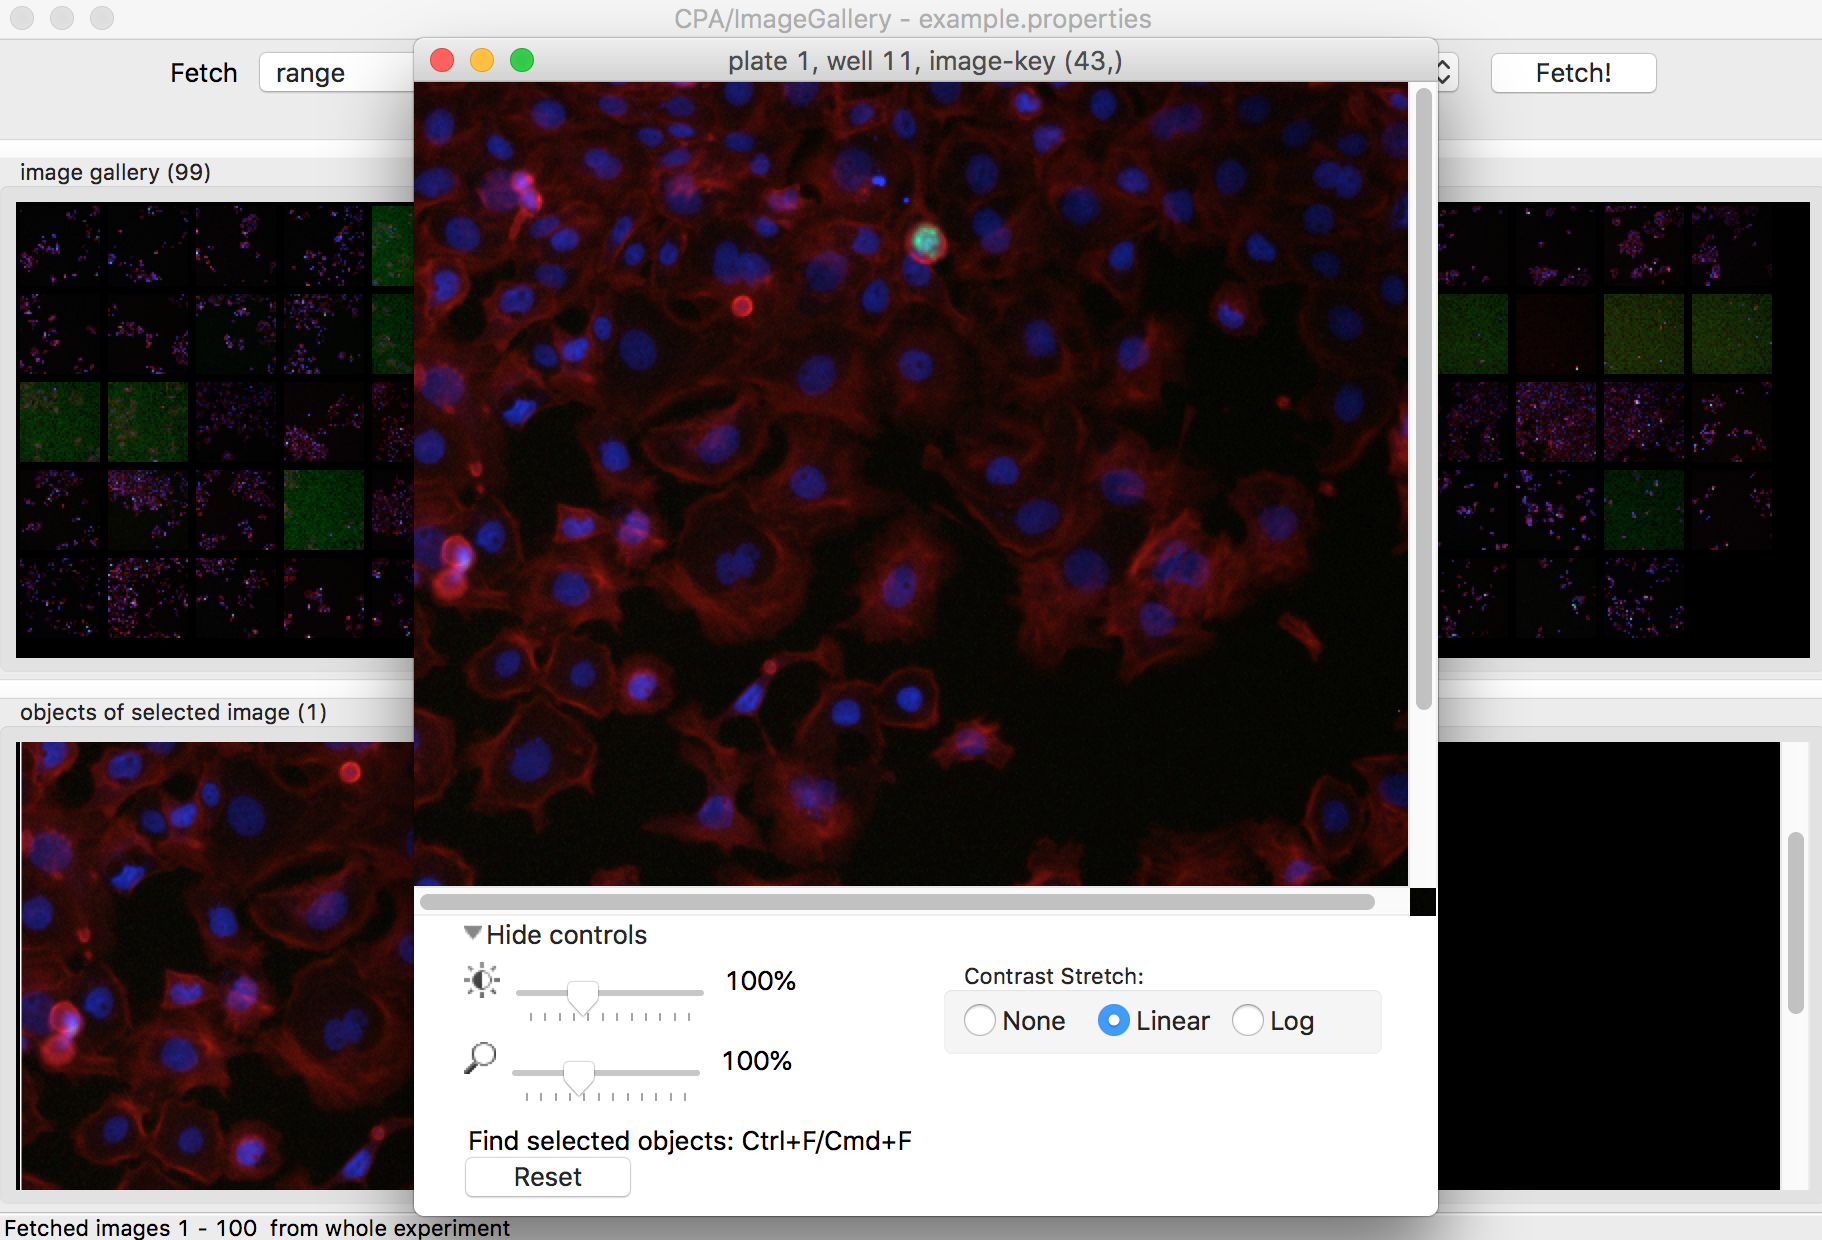
\includegraphics[width=1.0\linewidth]{bilder/related_work/visualization.png}
	\caption{CPA Main View Different Views Are Selectable (from \cite{Jones2008})}
	\label{fig:RL}
\end{figure}


\subsection{Downsides of CPA}
Getting CPA to run on a computer requires installation first. This installation is
not trivial as the system requires a MySQL database system to work.

Furthermore, the powerful user interface makes the system complex and difficult to use. This can 
scare off potential users.





